\newpage
\section{Uitvoerbaarheid Strategie\"{e}n}
\label{h6}

\subsection*{Deelvraag 3: Welke strategie is per specifieke bevolkingsgroep aan te bevelen wanneer zij de regel van van voorkeursdrempel in de kieswet te willen benutten in hun voordeel?}
Zoals in het vorige hoofdstuk al is beschreven kunnen de vier verschillende bevolkingsgroepen uit meerdere strate\"{e}n kiezen die een hoog rendement leveren. Daarmee lijkt de derde deelvraag makkelijk te beantwoorden. De bevolkingsgroepen kunnen simpelweg de strategie kiezen waarvan berekend is dat deze het hoogste rendement heeft. Of een strategie de voorkeur geniet boven een andere strategie ligt niet enkel aan het aantal zetels dat een strategie kan opleveren. Echter ligt de keuze voor een strategie ook aan een aantal andere factoren. Zo kan de uitvoering bemoeilijkt worden vanwege de wijze van uitvoering. Een bevolkingsgroep dient als collectief (ook wanneer enkel een deel van de bevolkingsgroep zich committeert) een strategie uit te voeren. Waar sommige Strategie\"{e}n makkelijk communiceerbaar zijn naar het grote publiek zijn andere Strategie\"{e}n moeilijker te communiceren. Echter is het mogelijk om d.m.v. informatie technologie (IT) een hulpmiddel in te schakelen waardoor een strategie nauwelijks gecommuniceerd dient te worden. Enkel het doel geniet dan nog relevantie en niet de wijze waarop het doel precies wordt bereikt. Derhalve zullen we verder kijken dan het rendement wat een strategie voor een bevolkingsgroep oplevert en zullen we de diepte in gaan d.m.v. twee subdeelvragen. \\
\indent In de eerste subdeelvraag gaan we onderzoeken hoe een strategie voor een bevolkingsgroep uitvoerbaar kan worden gemaakt. Hierbij gaan we onderzoeken hoe een strategie te communiceren is. De problematiek van het communiceren van een strategie ligt aan de complexiteit van een strategie. Er kan simpelweg niet verwacht worden dat alle leden van de bevolkingsgroep de regels van de strategie opvolgen wanneer de regels een zekere mate van complexiteit met zich mee brengen. Derhalve zullen we gebruik maken van IT om uitvoering van een strategie te realiseren. In de tweede subdeelvraag gaan we onderzoeken wat de eventuele voor- en nadelen kunnen zijn van de keuze voor de wijze van uitvoering van de strategie. Hierbij zullen we de voor- en nadelen tegen elkaar opwegen om zodoende proberen uit op een aanbeveling voor de wijze van uitvoering van een strategie.  


\subsection{Uitvoeringswijze Strategie\"{e}n.}

\subsection*{Subdeelvraag 3.1: Hoe kan een strategie uitvoerbaar worden gemaakt voor een specifieke bevolkingsgroep waarvan de leden zich willen committeren aan een strategie om de regel van de voorkeursdrempel te willen benutten in hun voordeel?}
In Hoofdstuk \ref{sec:eva} hebben we berekend hoeveel zetels onder leden van een bevolkingsgroep bedeeld hadden kunnen worden wanneer 100\% van de stemgerechtigde leden zich hadden gecommitteerd aan een strategie. In het vorige hoofdstuk hebben we vastgesteld dat zowel strategie 1 als strategie 2 voor elke bevolkingsgroep een hoog rendement oplevert. Echter van deze twee Strategie\"{e}n levert strategie 1, op de bevolkingsgroep allochtonen na, een hoger rendement op. Daarnaast is strategie 1 effici\"{e}nter in het verdelen van de stemmen (zie Hoofdstuk \ref{sec:eva}). Bij de bevolkingsgroep provincialen leverde echter strategie 4 het hoogste rendement op. Zowel strategie 1 als strategie 4 zijn echter moeilijk uit te voeren vanwege het feit dat de stemgerechtigde leden van een bevolkingsgroep op een \textit{N} kandidaten van de corresponderende bevolkingsgroep moeten stemmen. Hierbij wordt de \textit{N} bepaald door een serie aan regels (zie Sectie \ref{vrouwen} voor beschrijving van de regels) en dienen deze regels bekend te zijn bij de deelnemende leden van de bevolkingsgroep. Bij strategie 2 daarentegen moeten de deelnemende leden van de bevolkingsgroep enkel willekeurig op een kandidaat uit de corresponderende bevolkingsgroep stemmen. Bij de bevolkingsgroep vrouwen is dit vrij makkelijk. Op de kandidatenlijst van de partijen staat het geslacht van de kandidaten. Bij de andere bevolkingsgroepen is het echter lastiger om op een willekeurige kandidaat van de corresponderende bevolkingsgroep te stemmen. Op de kandidatenlijsten staat niet of iemand een allochtoon, een oudere of een provinciaal is. De woonplaats van de kandidaat staat niettemin wel vermeld. Echter, wil een provinciale kiezer op een provinciale kandidaat stemmen dan moet de kiezer weten of de woonplaats van de kiezer wel of niet in de Randstad ligt. Het wordt voor de bevolkingsgroepen allochtonen, ouderen en provincialen derha;ve niet alleen moeilijk om strategie 2 out te voeren maar ook om \"{u}berhaupt een strategie uit te voeren. \\
\indent Het uitvoeren en co\"{o}rdineren van strategie 1 bij de bevolkingsgroep vrouwen en het uitvoeren van welke strategie dan ook bij de andere bevolkingsgroepen is dus enigszins problematisch. Vanwege deze problematiek omtrent de uitvoering en co\"{o}rdinatie van de Strategie\"{e}n stellen we een tweetal IT-toepassingen voor. Deze toepassingen kunnen dienen als hulpmiddel voor de kiezers van alle vier de bevolkingsgroepen. Deze tweetal IT-toepassingen kunnen de kiezers assisteren bij het uitvoeren van een strategie. 

\paragraph{Hulpmiddel voor assistentie bij het kiezen van een willekeurige kandidaat.}
We stellen de eerste IT-toepassing voor die dient als hulpmiddel bij het kiezen van een willekeurige kandidaat conform alle in Hoofdstuk \ref{sec:eva} beschreven Strategie\"{e}n (bij alle Strategie\"{e}n moet er uiteindelijk willekeurig op een kandidaat gestemd worden). De toepassing kan al in een vrij simpele vorm bestaan zoals een website en mobiele website maar ook een mobiele applicatie behoort tot de mogeljkheden. Als voorbeeld hebben we echter gekozen voor een website. In Figuur \ref{fig:verkW} is een mock-up van de website te zien. Hierbij moet genoteerd worden dat de mock-up enkel dient om een beeld te scheten van hoe een hulpmiddel in de vorm van een website gebruikt zou kunnen worden. Er is hierbij geen aandacht besteedt aan het ontwerp en de gebruiksvriendelijkheid (usability) van de website. \\
\indent In de mock-up wordt strategie 2 uitgevoerd door de bevolkingsgroep allochtonen. De kiezer kiest de PVDA als de partij waarop zij/hij wilt gaan stemmen en de allochtone kandidaten op de kandidatenlijst van de PVDA worden getoond. De kiezer hoeft nu enkel willekeurig te kiezen uit één van de getoonde allochtone kandidaten. De kiezer kan deze keuze onthouden. Echter is er ook iets te bedenken waardoor de kiezer een reminder zou kunnen ontvangen in de vorm van een sms, een email etc. Het tonen van de foto van de kandidaat is af te raden. Kiezers kunnen op uiterlijk afgaan wanneer zij foto's van de mogelijk te kiezen kandidaten getoond krijgen \citep{banducci2008ballot,lawson2010looking}. \\


\begin{figure}[H]


	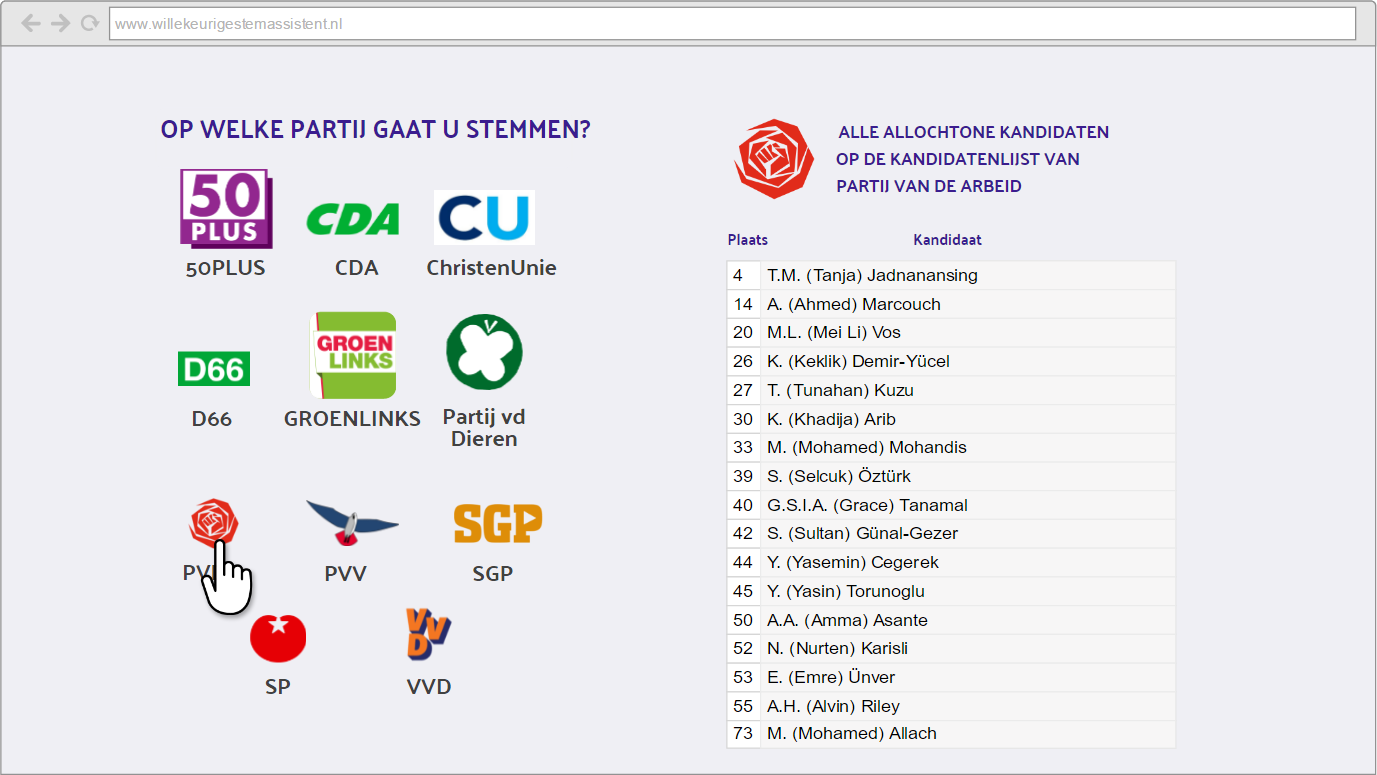
\includegraphics[width=\linewidth]{website_verkiezingen.png}

			\caption{Website als hulpmiddel die deelnemende leden kan helpen bij het kiezen van een willekeurige kandidaat uit de corresponderende bevolkingsgroep. Dit hulpmiddel kan ook bestaan in de vorm van een mobiele website en een mobiele applicatie.}

\label{fig:verkW}
\end{figure}

\paragraph{Hulpmiddel die willekeurige kandidaat uitkiest.}
We stellen de tweede IT-toepassing voor die dient als hulpmiddel bij het kiezen van een willekeurige kandidaat conform alle in Hoofdstuk \ref{fig:eva} beschreven Strategie\"{e}n. Ook deze toepassing kan al in een vrij simpele vorm bestaan zoals een website en mobiele website maar ook een mobiele applicatie behoort tot de mogelijkheden. Als voorbeeld hebben we echter gekozen voor een mobiele applicatie. In Figuur \ref{fig:verkA} is een mock-up van de mobiele applicatie te zien. Ook hierbij moet genoteerd worden dat de mock-up enkel dient om een beeld te scheten van hoe een hulpmiddel in de vorm van een mobiele website gebruikt zou kunnen worden. Er is hierbij geen aandacht besteedt aan het ontwerp en de gebruiksvriendelijkheid (usability) van de mobiele applicatie.\\
\indent In de mock-up wordt een strategie uitgevoerd door de bevolkingsgroep vrouwen. Voor het voorbeeld maakt het niet uit welke strategie dit is aangezien alle Strategie\"{e}n hierbij van toepassing zijn. In de mock-up in Figuur \ref{fig:verkA} kiest de kiezer voor GROENLNKS als de partij waarop zij (kan uiteraard ook een hij zijn als mannelijke kiezers willen deelnemen) wilt gaan stemmen en de mobiele applicatie wijst willekeurig een vrouwelijke kandidaat van GROENLINKS aan waarop de kiezer geacht wordt om de stem op uit te brengen. 


\begin{figure}[H]


	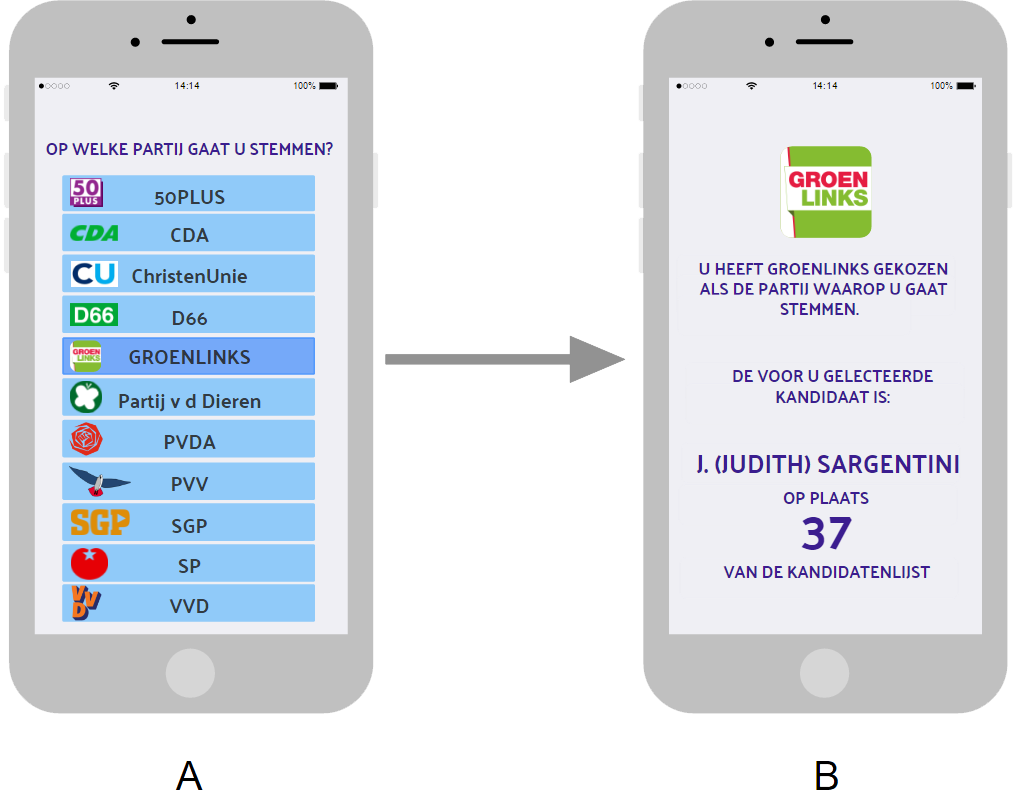
\includegraphics[width=\linewidth]{app_verkiezingen.png}

			\caption{Mobiele applicatie als hulpmiddel die een willekeurige kandidaat uitkiest. Dit hulpmiddel kan ook bestaan in de vorm van een mobiele website en een mobiele applicatie.}

\label{fig:verkA}
\end{figure}

In deze sectie hebben we gepoogd een antwoord te verschaffen op hoe een strategie uitgevoerd zou kunnen worden. Waar strategie 2 voor de bevolkingsgroep vrouwen gemakkelijk uitgevoerd kan worden en geen hulpmiddel aan te pas hoeft te komen, is de strategie voor de andere bevolkingsgroepen moeilijker uit te voeren. Een hulpmiddel in de vorm van een I-toepassing biedt uitkomst. In de volgende sectie gaan we de voor- en nadelen onderzoeken betreffende de keuze voor de wijze waarop een strategie zal worden uitgevoerd. 

\subsection{Voor- en nadelen van keuze voor een uitvoeringswijze strategie.}

\subsection*{Subdeelvraag 3.2: Wat zijn de eventuele voor- en nadelen van de keuze van de wijze waarop een strategie zal worden uitgevoerd?}
In de vorige sectie hebben we een tweetal IT-toepassingen voorgesteld die als hulpmiddel kunnen fungeren bij het uitvoeren van een strategie. Tevens hebben we opgemerkt dat strategie 2 voor de bevolkingsgroep vrouwen vrij gemakkelijk uit te voeren is. In deze sectie zullen we voor- en nadelen gaan onderzoeken van het kiezen voor een bepaalde uitvoeringswijze van een strategie. 

\paragraph{Hulpmiddel en geen hulpmiddel.} 
Vanwege de complexiteit die bij uitvoering van het merendeel van de Strategie\"{e}n om de hoek komt kijken hebben we een tweetal hulpmiddelen voorgesteld in de vorm van IT-toepassingen. Echter is het de vraag of er een behoefte zou zijn bij de deelnemende leden van de bevolkingsgroepen op de hulpmiddelen daadwerkelijk te gaan hanteren. \\
\indent Volgens de \textit{Information Richness Theory} \citep{daft1983information} willen mensen onzekerheid zoveel mogelijk pareren bij het uitvoeren van een taak. Hierbij is o.a. een directe terugkoppeling een belangrijk criteria. Voor uitvoering van alle Strategie\"{e}n is het dus zaak onzekerheid uit te sluiten wat betreft de mogelijke kandidaten waaruit gekozen dient te worden. Enkel bij strategie 2 bij de bevolkingsgroep vrouwen is er een directe terugkoppeling aanwezig om de kandidatenlijst. Bij strategie 2 moeten de kiezers willekeurig een corresponderende kandidaat kiezen en het geslacht van de kandidaat staat op de kandidatenlijst. Zodoende is bij uitvoering van strategie 2 door de bevolkingsgroep vrouwen geen hulpmiddel nodig. Bij de andere Strategie\"{e}n bij deze bevolkingsgroep moet er echter uit een top \textit{N} kandidaat worden gekozen (zie Hoofdstuk \ref{sec:eva}). Voor de andere strategie\"{e}n geldt dat er zowel geen directe terugkoppeling is te vinden op de kandidatenlijst (strategie 2) alsmede regels van de strategie te complex kunnen zijn om gemakkelijk toe te passen. \\
\indent Conform de \textit{Theory of Reasoned Action} \citep{fishbein1977belief,ajzen1991theory} en, in het verlengde van deze theorie, de \textit{Technology Acceptance Model} \citep{davis1989perceived,davis1989user, venkatesh2000determinants} zullen kiezers bereidwillig tegenover het gebruik van de technische hulpmiddelen staan wanneer deze hulpmiddelen de uit te voeren taak makkelijker maakt. Zodoende kan worden aangenomen dat in de meeste gevallen een hulpmiddel gewenst is bij het uitvoeren van een strategie. 

\paragraph{Keuze tussen een online of lokale database voor de mobiele applicatie.}
Wanneer een hulpmiddel in de vorm van een mobiele applicatie wordt gehanteerd zijn er enkele factoren wat betreft de data waar rekening mee gehouden dient te worden. Voor het verkrijgen van de data en de informatie tonen aan de gebruiker van de mobiele applicatie kan gekozen worden tussen een online database en een lokale database. Echter is ook beiden opties een mogelijkheid.  \\
\indent De online database zal een \textit{server/client} \citep{Chapt17:online} connectie opzetten waarbij de client de connectie met de server initieert en er data van de server naar de client en andersom gestuurd kan worden. Dit houdt in dat de gebruiker een internetconnectie dient te hebben om te zorgen dat de gewenste data actueel is en, in het geval van strategie 1 en 4, correspondeert met de laatste peilingen. Ook kan er voor gekozen worden om de keuze van de kiezer bij te houden in de database. Zo kunnen stemmen eventueel effic\"{e}nter gedistribueerd worden over de kandidaten. Echter is dit gevoelig voor manipulatie wanneer een persoon deze functionaliteit wil gebruiken om incorrecte data naar de database te sturen. Tevens is het de vraag of het ethisch verantwoord is om op deze manier bij te houden op welke partij een gebruiker stemt. \\
\indent Tegenover het gebruik van een online database staat het gebruik van een lokale database ge\"{i}mplementeerd in de mobiele applicatie. Voor een lokale database is geen internetconnectie nodig. De database wordt al simpelweg gevuld meegeleverd wanneer de mobiele applicatie wordt ge\"{i}nstalleerd. Een nadeel van een lokale database is echter dat de data in de database eventueel niet actueel is. Peilingen veranderen dagelijks en als een kiezer bijvoorbeeld tien dagen voor de verkiezingen de mobiele applicatie heeft ge\"{i}nstalleerd is de kans groot dat de data niet meer correspondeert met de laatste peilingen. Zodoende worden op de manier strategie 1 en strategie 4 waarschijnlijk niet optimaal uitgevoerd. \\
\indent Zowel een online database als een lokale database brengen voor- en nadelen met zich mee. Echter een combinatie van beiden kan uitkomst bieden. Een online database kan een lokale database vullen met de actuele data. Zodra de mobiele applicatie een internet connectie heeft opgezet kan de lokale database opnieuw opgevuld worden \citep{silberschatz1997database}. Ook in het geval dat de kiezer ten tijden van het gebruiken van de mobiele applicatie tijdens het uitbrengen van de stem geen internetconnectie heeft, kan de laatst opgehaalde data worden getoond aan de kiezer.


\paragraph{Willekeurige keuze van de kiezer vs. willekeurige toewijzing van een kandidaat aan de kiezer.} Bij het eerste voorgestelde hulpmiddel geeft de kiezer aan welke partij zij/hij wilt gaan stemmen waarna er een lijst wordt getoond met mogelijke kandidaten. Herbij wordt er vanuit gegaan dat de kiezer in staat is een willekeurige keuze te maken. Echter is het zo dat de mens inadequaat is als het gaat om willekeurige keuzes maken \cite{schulz2012analysing,bar1991perception,neuringer1986can}. Een computer is d.m.v. het toeassen van een \textit{Pseudorandom Number Generator} (PRNG) veel adequater in het willekeurig kiezen uit bijvoorbeeld een serie getallen of namen \cite{lewis1969pseudo,RANDO99:online,matsumoto1998mersenne,rukhin2001statistical}. Zodoende is het de vraag tot in hoeverre het aan de kiezer kan worden overgelaten om een willekeurige keuze te maken uit een lijst met namen zoals het geval zou zijn bij het gebruik van de eerst voorgesteld hulpmiddel. Bij het tweede voorgestelde hulpmiddel wordt  een kandidaat derhalve geselecteerd door de PRNG. Echter is het de vraag hoe kiezers reageren wanneer zij een kandidaat voorgeschoteld krijgen. Wanneer kiezers deze vorm verwerpen (bijvoorbeeld vanwege het gebrek aan keuzevrijheid) lijkt de eerste vorm voor een hulpmiddel meer geschikt. Hier is daarom aan te bevelen hier verder onderzoek naar te doen wanneer deze hulpmiddelen ontwikkeld gaan worden.  

\iffalse
\subsection{Beantwoording Deelvraag}
In deze sectie komen we nog even kort terug te komen op de deelvraag die in dit hoofdstuk is behandeld. De deelvraag luidde: welke strategie is per specifieke bevolkingsgroep aan te bevelen wanneer zij de regel van van voorkeursdrempel in de kieswet uit willen buiten in hun voordeel? Zoals al eerder gez
\fi
\newpage 